%%%%%%%% ICML 2020 EXAMPLE LATEX SUBMISSION FILE %%%%%%%%%%%%%%%%%

\documentclass{article}
\setlength\abovedisplayskip{3pt}
\setlength\belowdisplayskip{3pt}
% Recommended, but optional, packages for figures and better typesetting:
\usepackage{microtype}
\usepackage{graphicx}
%Path relative to the main .tex file 
\graphicspath{ {./images/} }
\usepackage{subfigure}
\usepackage{booktabs} % for professional tables
\usepackage{url}
\usepackage{calligra}
\usepackage{amsmath,amssymb,amsfonts}
\usepackage{caption}

% hyperref makes hyperlinks in the resulting PDF.
% If your build breaks (sometimes temporarily if a hyperlink spans a page)
% please comment out the following usepackage line and replace
% \usepackage{icml2020} with \usepackage[nohyperref]{icml2020} above.
\usepackage{hyperref}

% Attempt to make hyperref and algorithmic work together better:
\newcommand{\theHalgorithm}{\arabic{algorithm}}

% If accepted, instead use the following line for the camera-ready submission:
\usepackage[accepted]{icml2020}

% The \icmltitle you define below is probably too long as a header.
% Therefore, a short form for the running title is supplied here:
\icmltitlerunning{Standard Adversarial Training: Theory and Review}

\begin{document}

\twocolumn[
\icmltitle{Standard Adversarial Training: Theory and Review}

% It is OKAY to include author information, even for blind
% submissions: the style file will automatically remove it for you
% unless you've provided the [accepted] option to the icml2020
% package.

% List of affiliations: The first argument should be a (short)
% identifier you will use later to specify author affiliations
% Academic affiliations should list Department, University, City, Region, Country
% Industry affiliations should list Company, City, Region, Country

% You can specify symbols, otherwise they are numbered in order.
% Ideally, you should not use this facility. Affiliations will be numbered
% in order of appearance and this is the preferred way.
\icmlsetsymbol{}{*}

\begin{icmlauthorlist}
\icmlauthor{Moritz Sch\"uler}{to}
\end{icmlauthorlist}

\icmlaffiliation{to}{Department of Computer Science, Technical University of Munich, Munich, Germany}


\icmlcorrespondingauthor{Moritz Sch\"uler}{moritz.schueler@tum.de}

% You may provide any keywords that you
% find helpful for describing your paper; these are used to populate
% the "keywords" metadata in the PDF but will not be shown in the document
\icmlkeywords{Machine Learning, Robustness, Adversarial Training}

\vskip 0.3in
]

% this must go after the closing bracket ] following \twocolumn[ ...

% This command actually creates the footnote in the first column
% listing the affiliations and the copyright notice.
% The command takes one argument, which is text to display at the start of the footnote.
% The \icmlEqualContribution command is standard text for equal contribution.
% Remove it (just {}) if you do not need this facility.

\printAffiliationsAndNotice{}  % leave blank if no need to mention equal contribution


\begin{abstract}
 Adversarial training is a technique that tries to achieve robust deep networks. Robustness in a sense, that perturbing the input does not lead to a false prediction of the model. The presented paper provides a conceptual introduction to adversarial training as well as a review of current methods. While it's not possible to discuss all adversarial training approaches, some recent advancements are described in detail and their advantages and disadvantages are highlighted. Additionally, possible directions for future research are presented.
\end{abstract}

\vspace{-0.8cm}

\section{Introduction}
\label{Intro}
Many standard trained neural networks achieve high, even super human performance in a wide range of tasks. However, they can be easily fooled with the help of adversarial examples. Adversarial examples are generated by applying small perturbations to valid input data, which lead a classifier to change its prediction. Even though neural networks apply a non-linearity at each layer to allow for complex decision boundaries, \cite{b27} shows that the decision boundaries are excessively linear in most areas. This can be seen in figure \ref{fig1: Decision boundary of a neural network} for a trained CIFAR10 model. \\

\begin{figure}[H]
    \centering
    \vspace{-0.7cm}
    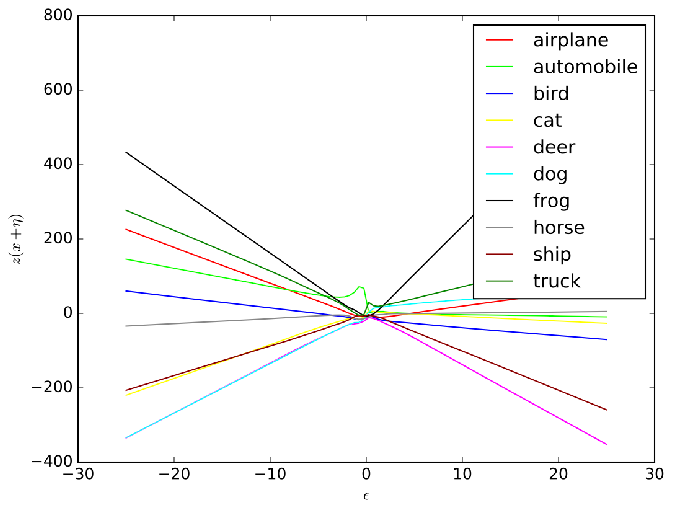
\includegraphics[scale=0.33]{CIFAR10-decision_boundary.png}
    \vspace{-0.35cm}
    \caption{Decision boundaries of a neural network trained on \\ CIFAR10 \cite{b27}}
    \label{fig1: Decision boundary of a neural network}
    \vspace{-0.2cm}
\end{figure}

Moreover, \cite{b2} demonstrated why linear decision boundaries are problematic for robustness. In figure \ref{fig2: standard and adversarial decision boundaries} on the left a perfect linear classifier is displayed. However, in the middle the presence of adversarial examples is shown. A small perturbation, bounded by shaded box around each sample, allows two samples to become adversarial (marked by a red star). Lastly, on the right a decision boundary for an adversarial trained network is displayed which is robust against small perturbations of the input data. Further, \cite{b6} demonstrated the need for robust models in practice, as simply putting a sticker on a stop sign fooled the network to recognize it as a speed limit. These problems lead to research how to defend against, but also how to generate adversarial examples. \\
  
\begin{figure}[ht]
  \centering
  \vspace{-0.6cm}
  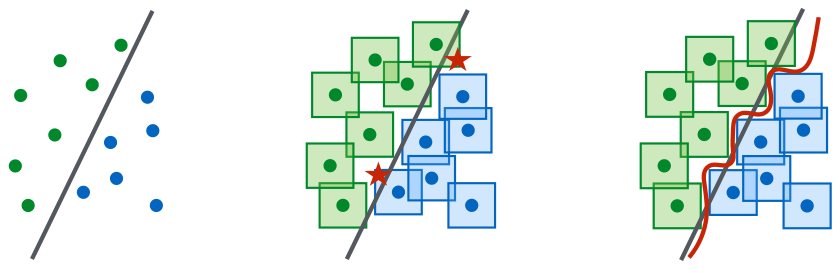
\includegraphics[scale=0.27]{decision_boundaries.png}
  \vspace{-0.45cm}
  \caption{"A conceptual illustration of standard vs. adversarial decision boundaries" \cite{b2}} 
  \label{fig2: standard and adversarial decision boundaries}
  \vspace{-0.2cm}
\end{figure}
\vspace{-0.07cm}
The latter one is called adversarial attack and focuses on finding a model that can generate adversarial examples by applying small perturbations to an input datapoint. Adversarial training on the other side is an approach to harden the model against adversarial attacks by training on adversarial examples of the input data. It tries to find perturbed samples that get wrongly classified, include them into the training and afterwards adjust the model parameters to get a correct prediction. In figure \ref{fig2: standard and adversarial decision boundaries} this means that the red classifier was trained with samples that lay on the edge of the surrounding boxes of the data points, leading to a robust decision boundary for these samples. \\
This paper aims at providing a comprehensive introduction to adversarial training and a review on current approaches. More precisely, it focuses on standard adversarial training, especially from the view of robust optimization. This includes universal adversarial training as well as margin maximization. However, there exist a variety of other approaches to increase the robustness of classifiers. The authors of \cite{b19, b20} use logit pairing, where a regularization is applied to the logits. \cite{b23} use ensemble methods to enhance robustness, whereas \cite{b21, b22} in contradiction distill the model. Another view on increasing robustness is calculating a distance within the prediction remains unchanged. This research area is about certifiable robustness \cite{b30}. Furthermore, latent representations are also examined to increase robustness \cite{b31}. \\
In the next section properties and types of adversarial attacks are presented. How to defend against them is part of the third section about the theoretical concept of adversarial training. Specific methods and their properties are shown in section 4, while section 5 gives a comparison of the discussed approaches. The last section specifies possible directions for future research.

\section{Adversarial Attacks}
  
The task of adversarial attacks is to find a model that generates samples for a given classifier, that are incorrectly classified. Let $x$ denote a sample from the distribution of the training data which classifies as $y$ with high probability $p(y|x)$. An adversarial example is now characterized by adding a small perturbation $\delta < \epsilon$ to $x$, such that the classification of $\tilde{x} = x + \delta$ results in $y'$ with high probability $p(y'|\tilde{x})$, but having a different predicted class $y' \neq y$. Here $\epsilon$ defines the maximum perturbation distance from the original sample, i.e. the boxes in figure \ref{fig2: standard and adversarial decision boundaries}. Another kind of adversarial example, not considered in this paper, is described by having a very large distance to the actual data distribution but still resulting in a high probability of $p(y'|\tilde{x})$. An example is to pass only random noise to trick the classifier. \\
The objective for adversarial attacks is to find a perturbation $\delta$, such that the loss of the classification model $l(f_{\theta}(x_i), y_i)$ is maximized. Usually a threat model $\Delta$ is used for this, which tries to find a $\delta$ within some $l_p$-norm smaller than $\epsilon$. Here $\epsilon$ is a hyperparameter that specifies the strength of the attack. 
\vspace{-0.2cm}
\begin{align*}
  \max_{\delta \in \Delta} & \quad l(f_{\theta}(x_i + \delta), y_i)  \\
  \Delta &= \{\delta : ||\delta||_p \leq \epsilon\} \quad \text{with} \quad \epsilon > 0
\end{align*}
Finding the maximum can easily be done via projected gradient ascent for the input $x$. However, accessing the gradient information is not always possible. This lead to the development of several different attacks. If a white box attack via gradient ascent is not feasible, the property that adversarial examples are model-agnostic can be used. The idea is to perform a gray box attack by training an own model on the data and using its gradient information to generate an attack. Lastly, if no gradient information is available at all, one can try to find gradient free perturbations, i.e. adding random noise and generate a black box attack. \\
Adversarial attacks can be further divided into targeted and non-targeted attacks. The first one tries to change the prediction of a given sample $x$ to a specified target label $y$, whereas the latter one only tries to change the prediction to some other class. Lastly, a distinction can be made between finding perturbation for each given sample $x$ or finding a single universal perturbation, that achieves a missclassification for many $x$. In this work, we focus on white box and non-targeted attacks, as for training the gradient is known and robustness should be increased generally and not for a specific class. 
  
\section{Adversarial Training}
  
Adversarial training is a training form for neural networks that tries to achieve higher robustness against adversarial attacks by using the adversarial examples belonging to the training data for training. By doing so it tries to increase the non-linearity of the decision boundary, as seen in figure \ref{fig2: standard and adversarial decision boundaries}. The training objective for adversarial training is a two step problem. Basically we are trying to minimize the loss of an adversarial attack model. \\
Let $x$ be a training sample and $f_{\theta}$ be the classifier, parametrized by $\theta$. First, we are solving a maximization of the classification loss, i.e. cross entropy loss, for a perturbation $\delta$ coming from a threat model $\Delta$ like in the case of an adversarial attack. This is done for each training sample separately and the "worst-case" losses are summed up. Afterwards, as in standard training, this summed loss is minimized via gradient descent on the model parameters $\theta$. This is done via mini-batches for several epochs as in usual training of neural networks.
\vspace{-0.2cm}
\begin{align}
  \label{eqn:saddle}
  \min_{\theta} & \sum_i \max_{\delta \in \Delta} \space l(f_{\theta}(x_i + \delta), y_i)  \\
  \Delta & = \{\delta : ||\delta||_p \leq \epsilon\} \quad \text{with} \quad \epsilon > 0
\end{align}
However, calculating the gradient of this objective function is not straight forward because of the max operation. By applying Daskin's Theorem the problem can be simplified. \\
\textbf{Danskin's Theorem}: The (sub)gradient of a function containing a max term can be found by taking the gradient at the point of the maximum $\delta^{*}$.
\begin{align*}
  \nabla_{\theta} \max_{||\delta|| \leq \epsilon} l(f_{\theta}(x_i + \delta), y_i) = \nabla_{\theta} l(f_{\theta}(x_i + \delta^{*}(x_i)), y_i)
\end{align*}
Theoretically, the theorem has some required conditions, which might not hold in the case of adversarial training, i.e. having a convex loss function $l(f_{\theta}(x_i + \delta), y_i)$ or that it only holds for the exact maximum. The trade-off emerging from that is, that the robustness depends on the precision of the maximum, but using a multi-step approach for a better approximation slows down the overall process. \\
The two main challenges, which are addressed by different presented methods in the next section are finding a better or faster solution for the generation of the adversarial training samples, as well as finding a way to be robust against all threat models. Because research showed that models are very robust against the threat model they were trained on, but lack robustness against other attacks.
  
\section{Methods}
  
In practice, several approaches have been studied to combat the mentioned challenges. In this section some recent methods and their peculiarities are presented. Especially the objective function, as well as the threat model used by the approaches are discussed.
  
\subsection{Robust Optimization - Standard Adversarial Training} \label{Robust Opti}
  
The standard approach on adversarial training stems from the view of robust optimization. It formulates the training process as a saddle point problem where the adversarial attack tries to maximize the loss whereas the network tries to minimize it. This is exactly the formulation presented in the previous section. Here we want to elaborate on the differences in threat models that are used to generate the adversarial examples. \\
The very first model was introduced by \cite{b9} in 2014, where the adversarial example $\tilde{x}$ is found by taking a single step into the gradient direction of defined length $\epsilon$. This technique is called fast gradient sign method (FGSM) and is the basis for most further optimization.
\begin{align*}
  \tilde{x} = x + \epsilon \cdot sgn(\nabla_x l(\theta,x,y)))
\end{align*}
The second threat model belonging to the family of robust optimization is the multi-step projected gradient descent method (K-PGD), created by \cite{b28}. Here instead of going a single big step into the gradient direction, we are moving $k$ (hyperparameter) smaller steps of size $\alpha$ into the gradient direction. Important is that if an update leads to stepping out of the $\epsilon$ ball, we need to project back, which is done by the projection function $\Pi$. This leads to a better approximation of the inner maximization but longer training times. 
\begin{align*}
    \tilde{x} &= \Pi (x + \alpha \cdot sgn(\nabla_x l(\theta,x,y)))
\end{align*}
Note that setting $k=1$ and $\alpha=\epsilon$ this resembles FGSM, so it can also be seen as a generalzation of the previous method. \\
Another approach that improves on FGSM brought in by \cite{b5} was Free Training. The main idea is to use the gradients from the outer minimization at time t for the gradient ascent of the adversarial example at time t+1. To reach a comparable robustness as K-PGD, each mini-batch is replayed $m$ times. Additionally, a new mini-batch is warm started by the perturbation of the previous one. To stay efficient the number of epochs is lowered accordingly, resulting in nearly no overhead compared to traditional training.
Fast Training, by \cite{b3}, further improved on Free Training by using FGSM with random initialization and getting rid of the mini-batch replay. They showed that the important ingredient to be comparably robust is only allowing for radomized initialization for the perturbation and thus could drastically speed up the training process. \\
% maybe put at the end of section or at beginning of comparison
Additionally, several training settings can influence the performance. Using another optimizer like momentum empirically leads to better adversarial examples \cite{b29}. Furthermore, increasing the capacity of a model can lead to improved robustness, as shown by \cite{b2}. Therefore, there is not a single approach that works for all problems. Instead, one should try different training setups, including different threat models.
  
\subsection{Universal Adversarial Training}
Universal Adversarial Training (UAT) is a method that does not try to find a perturbation for each single sample but rather a global perturbation that fools the classifier for many samples, hence the name universal. The difference can also be seen in the objective function which iterates over all samples in the inner term. As it tries to find a universal perturbation it is more constrained than the standard approach and hence leads to a less robust model, while reducing the training time. \\
In \cite{b4} the authors formulate this as a min-max optimization problem:
\begingroup
\setlength\abovedisplayskip{0pt}
\setlength\belowdisplayskip{6pt}
\begin{align}
  \label{eqn:universal}
  & \min_{\theta} \max_{\delta \in \Delta} \space \frac{1}{N} \sum_{i=1}^N \space \hat{l}(f_{\theta}(x_i + \delta), y_i) \\
  \text{with} \quad & \hat{l}(f_{\theta}(x_i + \delta), y_i) = \min \{l(f_{\theta}(x_i + \delta), y_i), \beta \}
\end{align}
\endgroup
where $\theta$ represents the trainable parameters of the neural network, $x_i$ the training samples, $y_i$ the training labels, $\delta$ the universal perturbation and $\hat{l}(\cdot)$ the loss function. Note, that $\delta$ is again bounded by an $l_p$-ball of size $\epsilon$. For this all presented models of the previous section can be used. Further notice, that the loss function $\hat{l}(\cdot)$ is bounded from above by a hyperparameter $\beta$. This is crucial because it hinders a single sample to dominate the average loss in the inner loop. Otherwise "a perturbation, that causes missclassification of just a single sample can maximize [the inner term] by forcing the average loss to infinity"\cite{b4}. \\
A recent advancement on this formulation is done by \cite{b11}. The key idea is to relax the constraints and thus get stronger attacks during training. Particularly, the authors show, a network trained on class-wise universal perturbations (CW UAT) exhibits higher robustness to universal perturbation attacks.
  
\subsection{Margin Maximization}
Margin Maximization is a method that tries to maximize the distance between each sample and its nearby decision boundary. Intuitively this makes the model more robust as an adversarial example is a slight perturbation of a datapoint that changes the model outcome and this is usually a sample that is very close to a decision boundary. Thus, by maximizing said distance, also called margin, it is harder to generate adversarial examples and therefore increasing robustness to adversarial attacks. \\
One formulation of the problem is given by \cite{b1}. Here the margin $d_\theta(x_i, y_i)$ is defined by the smallest successfull perturbation $\delta^*$, 
\begingroup
\setlength\abovedisplayskip{0pt}
\setlength\belowdisplayskip{6pt}
\begin{align*}
  d_\theta(x,y) & = ||\delta^*|| = min ||\delta|| \\ 
  \text{s.t.} \quad \delta: & L_\theta^{01}(x+\delta, y) = 1
\end{align*}
\endgroup
where $L_\theta^{01}$ is the 0-1 loss inidating a classification error. The idea, proposed by the authors, is to maximize the average margin over the data. Hence, they name it Max-Margin Adversarial training (MMA). For this, the problem is divided into maximizing the margin for already correctly classified samples $S_{\theta}^{+}$ and correcting the prediction for all wrongly classified datapoints in $S_{\theta}^{-}$.
\begin{align*}
  \min_{\theta} \Big\{ & \sum_{i \in S_{\theta}^{+}} \max \{0, d_{max} - d_\theta(x_i, y_i)\} \\ 
  & + \beta \sum_{j \in S_{\theta}^{-}} l_\theta (x_j, y_j) \Big\}
\end{align*}
Here $\beta$ controls the trade-off between maximizing the margin and correcting wrong predictions. $l(\cdot)$ is a standard classification loss, like cross entropy and $d_{max}$ is a hyperparameter, specifying the minimum margin we would like to achieve. Additionally, $d_{max}$ also leads the learning to focus on margins that are smaller as itself, because it acts as a threshold for the margin $d_\theta(x_i, y_i)$ inside the hinge loss. Finding the smallest margin in this work is done via a variant of K-PGD, presented in \ref{Robust Opti}.
  
\section{Review} \label{rev}
In this section the previously presented training methods are compared qualitatively based on their accuracy, robustness and training time. We also provide a quantitative comparison in the appendix, collected from the reviewed papers. Therefore, the numbers should be taken with caution because of i.e. different training setups. \\
The methods based on robust optimization try to solve a saddle point problem by alternating optimization of the inner and outer term of \ref{eqn:saddle}, which is costly computationally and time-wise. FGSM tries to mitigate this by only doing a single update on each sample, which is fast, but leads to a poor approximation of the maximum. Thus, making it harder to find the optimum and lowering the robustness. K-PGD on the other hand uses several smaller steps to approximate the maximum of the loss function, rendering it more robust as a better optimum can be found. However, the number of steps in the inner term massively increases the training time, resulting in limited usability for large and real world applications. With Free and Fast Training the idea is to keep the computational effiency of FGSM, while improving the robustness. Both techniques indeed achieve similar training times, but also lack a bit of robustness compared to K-PGD. \\
For the second group of methods, the idea was to find a single perturbation that works for all instances. This greatly speeds up the computation, as the inner term of \ref{eqn:universal} is only calculated once for each batch. On the other hand, having a single perturbation results in a weaker attack and lower robustness. Unfortunately, no statement regarding the robustness against usual white box attacks (i.e. PGD) can be made. But comparing the robust accuracies of models trained with UAT, class-wise UAT, FGSM and PGD against a threat model, that generates universal adversarial perturbations, shows that universally trained models can be equally robust and more efficient against those type of attack. Class-wise UAT outperforms standard UAT slightly, but also incorporates more training time, as an update per class needs to be found. \\
The third group of methods presented in this paper is trying to maximize the margin. For the MMA model, which approximates the minimal margin via multistep PGD a comparable robustness to K-PGD standard training can be achieved. However, using multiple iteration increases the training time.
  
\section{Future Research}
Standard adversarial training generally faces a trade-off between the precision and the speed of finding the maximum. Hence, the key question that will remain is how to find a fast way to construct adversarial examples without sacrificing robustness. Additionally, the generalization of training methods to be robust against different threat models remains open. Especially challenging is, that generally it is easier and faster to use a new and promising threat model to construct a single adversarial example than it is to use a sophisticated approach to train a classifier against it. \\
As it is important to focus on finding better threat models, the training setup itself already incorporates high variance, therefore it might be a good idea to compare the models over a wide variety of hyperparameters and datasets to get a fair assessment of the advancements. Also, the majority of proposed solutions re-uses neural network architectures build solely for high accuracy, completely disregarding robustness. Therefore, it might be interesting to determine new architectures, specifically designed for robustness. \\
Even though adversarial training is a good step for increased robustness, a general important step is to further increase the understanding of the predictions of neural networks by the use of explainable AI. Because adversarial examples showed that the interpretation of a scene for neural networks is completely different to that of a human, and robust models might still be vulnerable to a new kind of attack.  

\newpage

\appendix
\section{Quantitative comparison of adversarial trained models on CIFAR10}
The following table contains quantitative results from models trained on CIFAR10 to support the comparisons of the presented methods in section \ref{rev} of this paper. Again, be careful to rank those approaches only by numbers, as the training setup, as well as the attack model differ between papers. Below the table the differences in training are summarized. To check the precise parameters and architectures the papers are linked.
\vspace*{-0.2cm}

\begin{table}[!htbp]
  \centering
  \caption{Evaluation of different methods used to do adversarial training on CIFAR10}
  \vspace*{-0.2cm}
  \begin{center}
  \resizebox{\columnwidth}{!}{
  \begin{tabular}{|c|c|c|c|c|}
  \hline
  &\multicolumn{4}{|c|}{\textbf{Evaluation criteria}} \\
  \cline{2-5} 
  {\textbf{Method}} & \textbf{Clean} & \textbf{PGD} & \textbf{Combined} & \textbf{Training} \\
  & \textbf{Accuracy} & \textbf{($\epsilon=8/255$)} & \textbf{Accuracy{$^{\mathrm{1}}$}} & \textbf{Time (min)} \\
  \hline
  FGSM{$^{\mathrm{2}}$} & 85.18\% & 0.00\% & 42.59\% & 12.37 \\
  7-PGD{$^{\mathrm{3}}$} & 82.46\% & 50.69\% & 66.58\% & 68.8 \\
  Free (m=8){$^{\mathrm{4}}$} & 78.38\% & 46.18\% & 62.28\% & 20.91 \\
  Fast{$^{\mathrm{2}}$} & 85.32\% & 44.01\% & 64.67\% & 12.33 \\
  \hline
  8-PGD{$^{\mathrm{5}}$} & 85.14\% & 46.47\% & 65.81\% & - \\
  MMA-20{$^{\mathrm{5}}$} & 86.56\% & 46.89\% & 66.73\% & - \\
  \hline
  & & IFGSM (k=10) & & \\
  Large Margin{$^{\mathrm{6}}$} & ~90.00\% & ~52.00\% & 71.00\% & - \\
  \hline
  & & UAP{$^{\mathrm{7}}$} & & \\
  \hline
  Baseline{$^{\mathrm{8}}$} & 96.20\% & 20.20\% & 58.20\% & - \\
  FGSM{$^{\mathrm{9}}$} & 91.42\% & 51.00\% & 71.21\% & - \\
  PGD{$^{\mathrm{8}}$} & 86.80\% & 86.10\% & 86.45\% & - \\
  UAT{$^{\mathrm{8}}$} & 94.40\% & 89.80\% & 92.10\% & - \\
  CW UAT{$^{\mathrm{8}}$} & 94.90\% & 94.80\% & 94.85\% & - \\
  \hline
  \multicolumn{5}{l}{$^{\mathrm{1}}$Average over Clean Accuracy and Accuracy for the attack} \\
  \multicolumn{5}{l}{$^{\mathrm{2}}$As reported by \cite{b3}. The adversary does 50 iterations with} \\
  \multicolumn{5}{l}{$\quad$ 10 random restarts and $\alpha=2/255$} \\
  \multicolumn{5}{l}{$^{\mathrm{3}}$As reported by \cite{b28}. The adversary does 20 iterations with} \\
  \multicolumn{5}{l}{$\quad$ zero random restarts and $\alpha=2/255$} \\
  \multicolumn{5}{l}{$^{\mathrm{4}}$As reported by \cite{b5}. The adversary does 20 iterations with} \\
  \multicolumn{5}{l}{$\quad$ 10 random restarts and $\alpha=2/255$} \\
  \multicolumn{5}{l}{$^{\mathrm{5}}$As reported by \cite{b1}} \\
  \multicolumn{5}{l}{$^{\mathrm{6}}$As reported by \cite{b15}. Note, that a different attack model is used} \\
  \multicolumn{5}{l}{$\quad$ and the values are determined from the plots in the paper} \\
  \multicolumn{5}{l}{$^{\mathrm{7}}$Note, that a different attack model by \cite{b10} is used here} \\
  \multicolumn{5}{l}{$^{\mathrm{8}}$As reported by \cite{b11}. The adversary does 7 iterations} \\
  \multicolumn{5}{l}{$^{\mathrm{9}}$As reported by \cite{b4}. Note that settings aren't exactly the same} \\ 
  \multicolumn{5}{l}{$\quad$ as in \cite{b11}, but comparable}
  \label{tab:modeleval}
  \end{tabular}
  }
  \label{tab1}
  \end{center}
\end{table}
\vspace*{-0.3cm}

The results of the first part of the table stem are all contained in \cite{b3}. For the training they used a batch size of 128, momentum as optimizer and a weight decay of $5 \cdot 10^{-4}$. A key difference for the values of Fast and Free training is, that the adversary for Fast training is stronger and Free training utilized a different network architecture. Fast uses a ResNet, whereas the authors of Free decided for a WideResNet model. Also they use a batch size of 256 \cite{b5}. Unfortunately, for \cite{b28} no exact details are known for the training procedure. For the margin based training, the architecture is a WideResNet as well \cite{b1}. To optimize the parameters SGD with momentum update rule with weight decay was instantiated. Each batch contained 128 images and a fixed learning rate schedule was proposed. The same settings are also used by \cite{b4}, however the used architecture is not mentioned. The class-wise UAT method again uses a WideResNet architecture \cite{b11}, but does not specify further training parameters. \\
From the short overview, it can be seen that many methods used similar training setups. However, these small differences might be enough to lead to unfair results. Changing the optimizer to momentum improved generation of adversarial examples for already available methods by quite a bit \cite{b29}. Therefore, it is unclear how strong the training settings influence the robustness of the presented approaches. Furthermore, the values are intriguing, as by only looking at the values, it seems that class-wise UAT is the best model. But the accuracy is achieved on a different attack model, which is more limited than that the PGD adversary, thus weaker. To get reliable and fair values the experiments have to be repeated by a single instance, s.t. training parameters, as well as, adversarial attack model are unified.

\newpage

\bibliographystyle{icml2020}

\begin{thebibliography}{00}

    \bibitem{b1} Gavin Weiguang Ding, Yash Sharma, Kry Yik Chau Lui, Ruitong Huang: MMA Training: Direct input space margin maximization through adversarial training. 2019.
    \bibitem{b2} Aleksander Madry, Aleksandar Makelov, Ludwig Schmidt et al.: Towards Deep Learning Models Resistant to Adversarial Attacks. 2019.
    \bibitem{b3} Eric Wong, Leslie Rice, J. Zico Kolter: Fast is better than Free: Revisiting adversarial training. 2020.
    \bibitem{b4} Ali Shafahi, Mahyar Najibi, Zheng Xu et al. Universal Adversarial Training. 2020.
    \bibitem{b5} Ali Shafahi, Mahyar Najibi, Amin Ghiasi, Zheng Xu, John Dickerson, Christoph Studer, Larry S Davis, Gavin Taylor, and Tom Goldstein. Adversarial training for free! 2019.
    \bibitem{b6} Eykholt, K., Evtimov, I., Fernande, E., Li, B., Rahmati, A., Xiao, C., Prakash, A., Kohno, T., and Song, D. Robust physicalworld attacks on deep learning visual classification. 2018.
    \bibitem{b9} Ian J Goodfellow, Jonathon Shlens, and Christian Szegedy. Explaining and harnessing adversarial examples. 2014.
    \bibitem{b10} Seyed-Mohsen Moosavi-Dezfooli, Alhussein Fawzi, Omar Fawzi,Pascal Frossard. Universal adversarial perturbations. 2017.
    \bibitem{b11} Philipp Benz, Chaoning Zhang, Adil Karjauv, In So Kweon. Universal adversarial training with class-wise perturbations. 2021.
    \bibitem{b15} Gamaleldin F. Elsayed, Dilip Krishnan, Hossein Mobahi, Kevin Regan, Samy Bengio. Large Margin Deep Networks for Classification. 2018.
    \bibitem{b19} Harini Kannan, Alexey Kurakin, Ian Goodfellow. Adversarial Logit Pairing. 2018.
    \bibitem{b20} Marius Mosbach, Maksym Andriushchenko, Thomas Trost, Matthias Hein, Dietrich Klakow. Logit Pairing Methods Can Fool Gradient-Based Attacks. 2019.
    \bibitem{b21} Nicolas Papernot, Patrick McDaniel, Xi Wu, Somesh Jha, Ananthram Swami. Distillation as a Defense to Adversarial Perturbations against Deep Neural Networks. 2016.
    \bibitem{b22} Nicholas Carlini, David Wagner. Defensive Distillation is Not Robust to Adversarial Examples. 2016.
    \bibitem{b23} Florian Tramèr, Alexey Kurakin, Nicolas Papernot, Ian Goodfellow, Dan Boneh, Partick McDaniel. Ensemble Adversarial Training: Attacks and Defenses. 2020.
    \bibitem{b27} Ian Goodfellow. Adversarial Examples and Adversarial Training. 2016. "\url{https://berkeley-deep-learning.github.io/cs294-dl-f16/slides/2016_10_5_CS294-131.pdf}". Accessed: 27.05.2021
    \bibitem{b28} Aleksander Madry, Aleksandar Makelov, Ludwig Schmidt, Dimitris Tsipras, and Adrian Vladu. Towards deep learning models resistant to adversarial attacks. ICLR, 2017.
    \bibitem{b29} Yinpeng Dong, Fangzhou Liao, Tianyu Pang, Hang Su, Jun Zhu, Xiaolin Hu, and Jianguo Li. Boosting adversarial attacks with momentum. 2018.
    \bibitem{b30} Jeremy Cohen, Elan Rosenfeld, J. Zico Kolter. Certified Adversarial Robustness via Randomized Smoothing. 2019.
    \bibitem{b31} Pouya Samangouei, Maya Kabkab, Rama Chellappa. Defense-GAN: Protecting Classifiers against Adversarial Attacks using Generative Models. 2018.
  
  \end{thebibliography}

\end{document}
